\section{GSM \formelbuch{242}}
	\begin{center}
	\begin{tabular}{|l|l|l|l|l|} \hline
	          & GSM850     & GSM900        & GSM1800 (DCS)       & GSM1900 (PCS) \\ \hline  \hline
	uplink freq.
	   &  824--849\,MHz & 890--915\,MHz & 1710--1785\,MHz & 1850--1910\,MHz \\ \hline
	downlink freq. 
	   & 869–894\,MHz  & 935--960\,MHz & 1805--1880\,MHz & 1930--1990\,MHz \\ \hline
	duplex separation 
	   &  45\,MHz & 45\,MHz & 95\,MHz & 80\,MHz \\ \hline
	\# RF channels 
	   & 124  & 124 & 374 & 299 \\ \hline
	avg. MS transmission power 
	   & - & 250\,mW & 125\,mW & 125\,mW \\ \hline
	peak MS transmission power 
	   & -  & 2\,W & 1\,W & 1\,W \\ \hline
	\end{tabular} \\
	HF Parameter von verschiedenen GSM Systemen
	\end{center}

    \begin{minipage}{7.4cm}    
	    \begin{center}
	    \begin{tabular}{|l|l|} \hline
	    name & value \\ \hline \hline
	    access method           & TDMA-FDD \\ \hline
	    multiplex number        & 8 \\ \hline
	    TDMA frame length       & 4.615\,ms \\ \hline
	    channel spacing         & 200\,kHz \\ \hline
	    bit rate                & 270.833\,kbps \\ \hline
	    bit duration            & 3.7\,$\mu$s \\ \hline
	    modulation type         & GMSK, BT$=0.3$ \\ \hline
	    user data transfer rate & 2.4, 4.8, or 9.6\,kbps \\ \hline
	    channel equalization    & up to 16\,$\mu$s \\ \hline
	    \end{tabular} \\
	        Systemparameter von GSM
	    \end{center}
    \end{minipage}
    \begin{minipage}{2cm}        
        \quad
    \end{minipage}
    \begin{minipage}{9cm}    
        \footnotesize
        Uplink(Mobile TX)- \& Downlink(Base TX)-Timeslots sind zeitlich verschoben
        $\Rightarrow$ nur 1 Synthesizer und wenig steileres Filter nötig!
        \normalsize    \\
        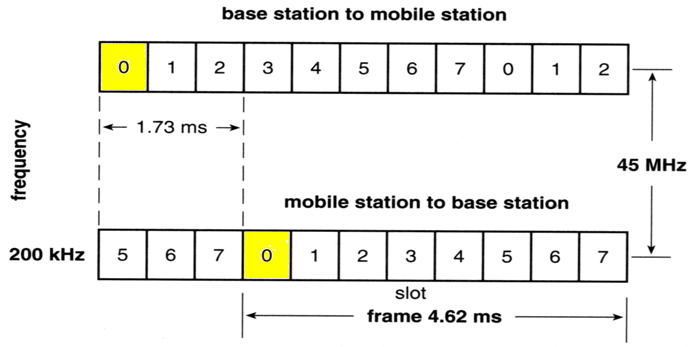
\includegraphics[width=8.5cm]{./bilder/systems-gsm-ud-slots.png}
    \end{minipage}

    \begin{minipage}{6.5cm}        
        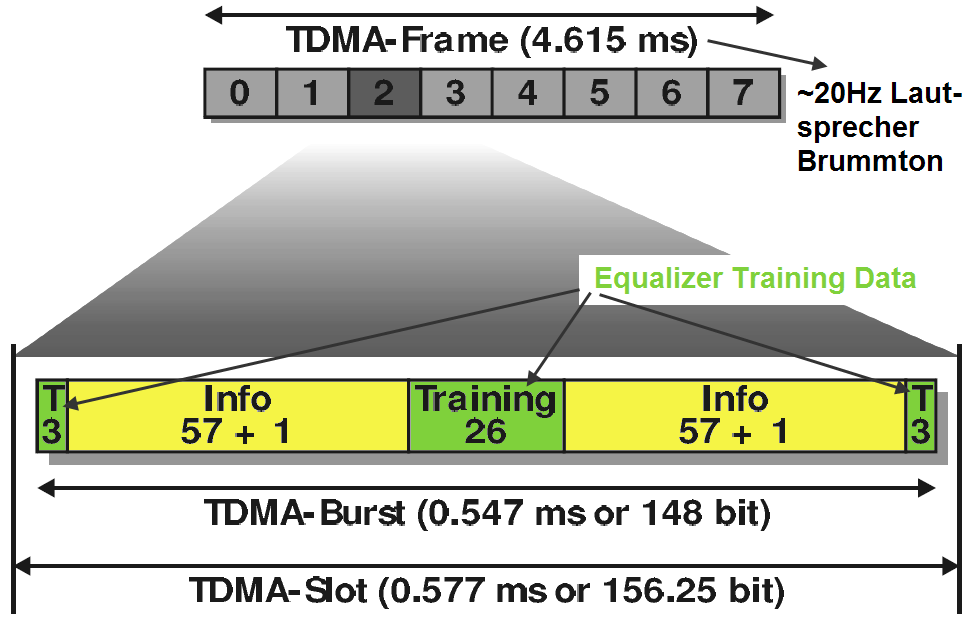
\includegraphics[width=6.5cm]{./bilder/systems-tdma.png} \\
        Not shown in picture above: Guard Period of 8.25 symbol required to overcome the 550m of TA tolerance.
    \end{minipage}
    \begin{minipage}{0.5cm}        
        \quad
    \end{minipage}
    \begin{minipage}{5.4cm} 
         \small
        Verwendung von benachbarten Kanälen (bspw.: CH0 \& CH1) ist in benachbarten Zellen nicht gestattet, weil ein
        Dynamic Range von $\pm 70$ dB gewährleistet werden muss. Deshalb muss immer ein Kanal übersprungen werden. 
        (bspw.: CH0 \& CH2 nutzen). \\
        Die Up- \& Downlinkfreq. $f_{\text{u}},f_{\text{d}}$ sind durch die Kanalnummer $n$ gegeben:
            $$f_{\text{u}}(n)=890\text{MHz} + 200\text{kHz}\cdot n$$
            $$f_{\text{d}}(n)=f_{\text{u}}(n)+45\text{MHz}$$
        \normalsize
    \end{minipage}
    \begin{minipage}{6.5cm}        
        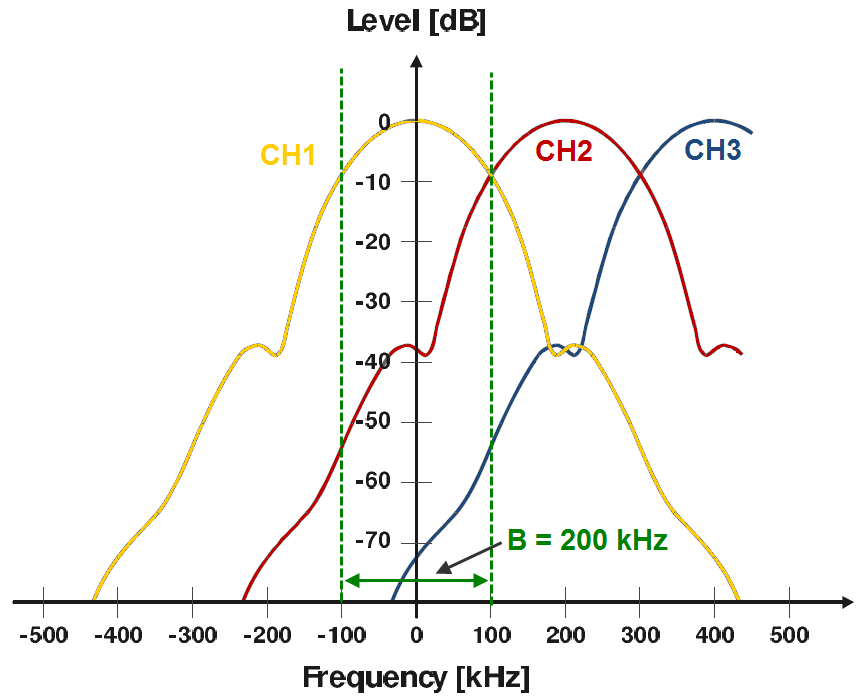
\includegraphics[width=6.5cm]{./bilder/systems-gsm-spectrum.png}
    \end{minipage}

	Damit auch die Signale von weiter entfernten MS innerhalb des zugehörigen Zeitschlitzes bei der BS ankommen, wird 
	dem MS die Zeitverschiebung (TA, Timing Advance) mitgeteilt. Der TA kann 64 Werte haben wobei 1 Bit ($T_B=3.69$\,$\mu$s) einer 
	Distanz von ca. 550m zur BTS entspricht (z.B. ein $\text{TA}=63$ entspricht $63 \cdot 550\text{m} = 35\text{km}$ Distanz zwischen MS und BS).

\subsection{Logische Kanäle und Bursts}
    Die Datenübertragung und Signalisierung zwischen MS (Mobile Station) und BS (Base Station) ist in 11 Kanäle 
    unterteilt.
    \begin{liste}
        \item \textbf{TCH/F, TCH/H}: Datenkanäle mit unterschiedlichen Geschwindigkeiten (siehe Tabelle unten).
        \item \textbf{FCCH}: Sendet den  Frequency Corr. Burst (Konstante Frequenz) und dient zur Justierung der BS-Frequenz beim MS.
        \item \textbf{SCH}: Ermöglicht MS die Synchronisation von Frame- \& Samplezeit, Identifiziert die BS
        \item \textbf{BCCH}: Sendet Zellen- und Netzwerkinformation. Wird von jeder BS immer mit maximaler Leistung gesendet!
        \item \textbf{RACH}: Ermöglicht MS an BS zu senden. Funktioniert nach ALOAH Zugriffsverfahren.
    \end{liste}

    \begin{center}    
        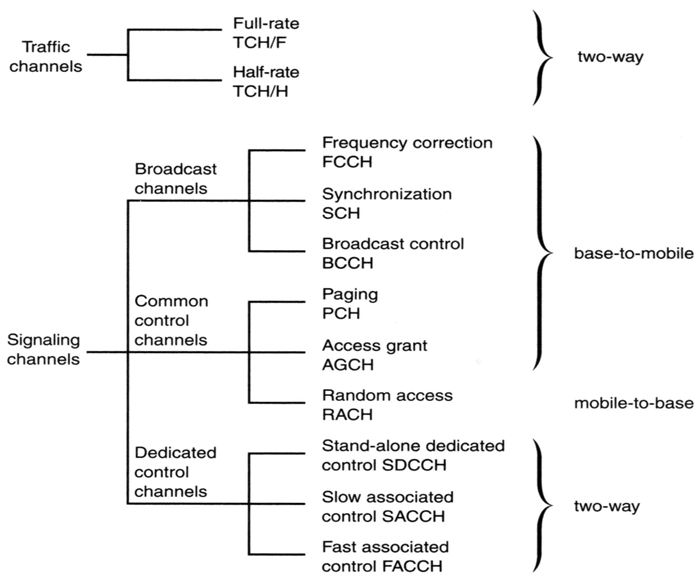
\includegraphics[height=7cm]{./bilder/systems-gsm-logicalCH.png}
	    \hspace{1cm}
        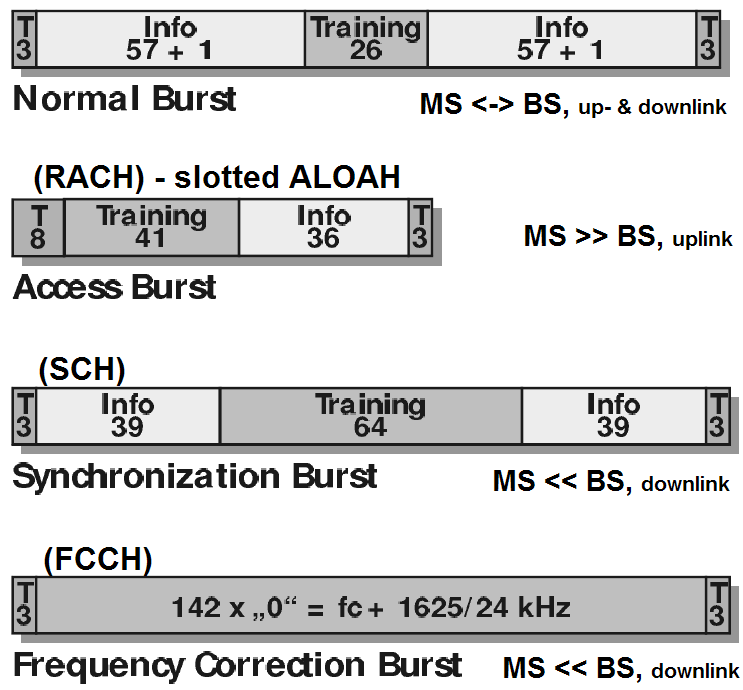
\includegraphics[height=7cm]{./bilder/systems-gsm-bursts.png}
    \end{center}

    \begin{minipage}{7.3cm}        
        \begin{center}
	        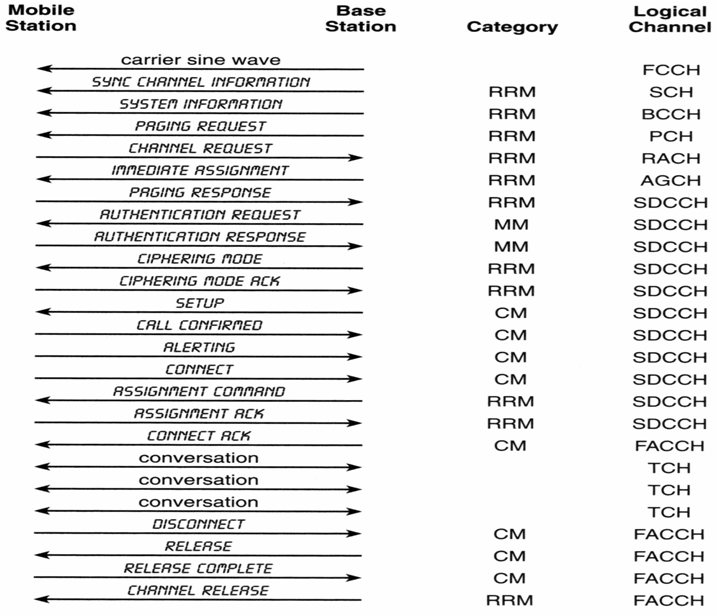
\includegraphics[width=7cm]{./bilder/systems-callEstablishment.png}    \\
	        Sequenzdiagramm eines Anrufs            
        \end{center}    
    \end{minipage}
    \begin{minipage}{12cm}  
        Grundsätzlich gilt, je tiefer die codierte Bitrate, desto störsicherer der Datenkanal und
        umgekehrt. Bits, welche bei der codierten Bitrate fehlen, werden für die Fehlererkennung \&
        - korrektur eingesetzt. 
        \begin{center}
            \small       
            \begin{tabular}{|l|l|r|r|}\hline
            abbr.     & name       & coded bitrate & raw bitrate \\ \hline \hline
            \multicolumn{4}{|l|}{\bf Full-rate TCH} \\ \hline
            TCH/FS    & full-rate speech channel & 13\,kb/s & 22.8\,kb/s \\ \hline
            TCH/F9.6  & full-rate data channel for 9600\,bps
                      & 9.6\,kb/s & 22.8\,kb/s \\ \hline
            TCH/F4.8  & full-rate data channel for 4800\,bps
                      & 4.8\,kb/s & 22.8\,kb/s \\ \hline
            TCH/F2.4  & full-rate data channel for 2400\,bps
                      & 2.4\,kb/s & 22.8\,kb/s \\ \hline \hline
            \multicolumn{4}{|l|}{\bf Half-rate TCH} \\ \hline
            TCH/HS    & half-rate speech channel & 6.5\,kb/s & 11.4\,kb/s \\ \hline
            TCH/H4.8  & half-rate data channel for 4800\,bps
                      & 4.8\,kb/s & 11.4\,kb/s \\ \hline
            TCH/H2.4  & half-rate data channel for 2400\,bps
                      & 2.4\,kb/s & 11.4\,kb/s \\ \hline 
            \end{tabular} \\
            Verschiedene Datenkanäle in GSM
            \normalsize
        \end{center}          
    \end{minipage}


\subsection{Handset Architekturen \formelbuch{252}}
    \begin{minipage}{7cm} 
      Man unterscheidet verschiedene Typen von Handsets: 
      \begin{liste}
        \item Standard - Singleband (nur 900 MHz)
        \item Multiband - Dual-, Tri- \& Quadband
        \item Multimode - mit DECT od. SAT Modus
        \item SDR (Software-Defined Radio) - 
                wie GNU Radio, unerwünscht von Herstellern,
                weil nur neue SW und nicht HW verkauft wird.
      \end{liste}
    \end{minipage}
    \begin{minipage}{12cm}    
        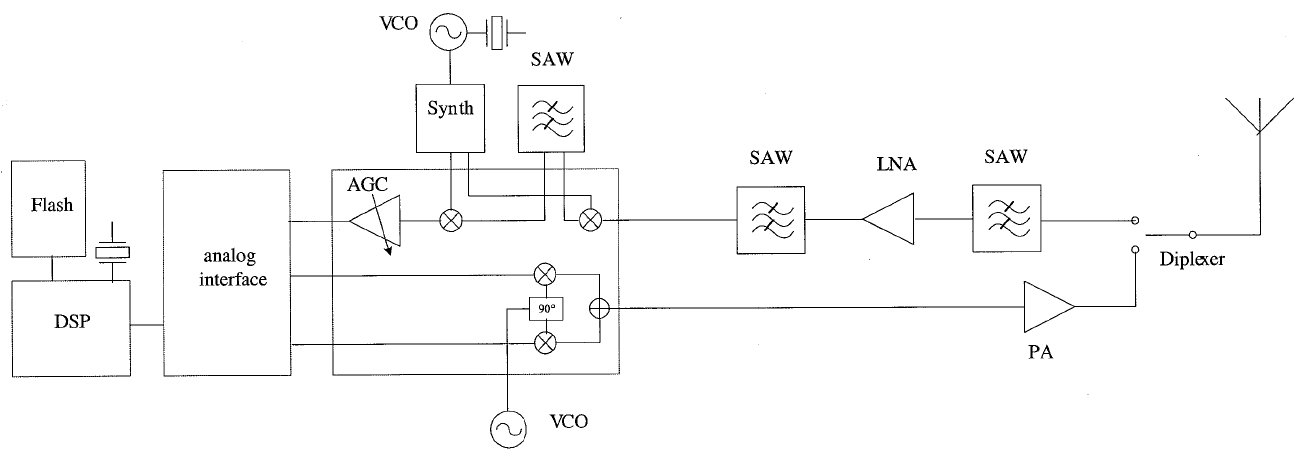
\includegraphics[width=12cm]{./bilder/systems-handset.png}
    \end{minipage}

